\documentclass[12pt,a4paper]{article}
\usepackage[utf8]{inputenc}
\usepackage{amsmath}
\usepackage{amsfonts}
\usepackage{amssymb}
\usepackage{graphicx}
\usepackage{physics}
\usepackage{float}
\usepackage[margin=1in]{geometry}
\usepackage{enumitem}
\usepackage{breqn}
\usepackage{soul, color}
\usepackage{blindtext}
\usepackage{mathtools}
\usepackage{verbatim}
\begin{document}
\title{ Calculating the Shear Modulus of our Vertex Model }
\author{Avik Mondal}
\maketitle
\section{Introduction}
%We're trying to come up with a way to calculate the shear modulus in the limit that the shear is $0$ (where we analytically calculate an equation instead of applying a small shear to the tissue). For all of these, we need to calculate the Hessian. 

Use theory from New Journal of Physics paper by Manning and Merkel from 2018. Don't forget, all the energies below have to be nondimensionalized before you implement any calculations. 

\section{Starting from the Energy}
We can begin at the very beginning to establish notation.

\begin{align}
	\label{eqn: hamiltonian}
	E = \sum\limits_{\alpha=1}^{F} \frac{1}{2} K (A_\alpha - A_0)^2 + \frac{1}{2} \Gamma(P_\alpha - P_0)^2
\end{align}
We sum over cells $\alpha$ where $F$ is the number of cells (faces). We know the first derivative of this energy is:

\begin{align}
	\label{eqn: negativeforce}
	\pdv{E}{r_i^\mu} = \sum\limits_{\alpha=1}^{F} K (A_\alpha- A_0) \pdv{A_\alpha}{r_i^\mu} + \Gamma(P_\alpha - P_0)\pdv{P_\alpha}{r_i^\mu}
\end{align}

Here, I use $\mu$ to represent components (x and y) and the Roman lowercase symbols to indicate vertex indices. For the second derivative, I will add $\nu$ to take the value of $x$ or $y$ and $j$ to indicate vertex indices.

\begin{align}
	\label{eqn: Hessian1}
	\pdv[2]{E}{r_j^\nu}{r_i^\mu} &= \sum\limits_{\alpha=1}^{F}K \pdv{A_\alpha}{r_j^\nu} \pdv{A_\alpha}{r_i^\mu} + K (A_\alpha - A_0) \pdv[2]{A_\alpha}{r_j^\nu}{r_i^\mu} + \Gamma \pdv{P_\alpha}{r_j^\nu} \pdv{P_\alpha}{r_i^\mu} + \Gamma (P_\alpha - P_0)  \pdv[2]{P_{\alpha}}{r_j^\nu}{r_i^\mu} \\
	= H_{ij}^{\mu \nu}
\end{align}
\section{The double derivatives}

The single derivatives are already known. The double derivatives are trickier and we have not yet calculated them before (10/11/2023). So let's derive them here:

\subsection{Area}

\begin{align}
	\label{eqn: firstareaderivative}
	\pdv{A_\alpha}{r_i^\mu} &= \pdv{r_i^\mu} \frac{1}{2} \sum\limits_{i=1}^V \hat{z}\cdot(\vb{r}_{i+1} \times \vb{r}_i)\\
	&= \frac{1}{2} \Big[\hat{z} \times  \big(\vb{r}_{i+1, i-1}\big)\Big]\cdot\widehat{\mu}
\end{align}
We start by defining the area with the shoelace formula. The ``+1" refers to a counterclockwise traversal of the polygon.$\widehat{\mu}$ refers to the unit vector corresponding to index $\mu$ (i.e. if $\mu = 1$, then $\widehat{\mu} = \hat{x}$).  In the above formulation:
\begin{align}
	\vb{r}_{i+1,i-1} = \vb{r}_{i+1} - \vb{r}_{i-1}
\end{align}
So then the second derivative follows straightforwardly from Eqn. \ref{eqn: firstareaderivative}:

\begin{align}
	\label{eqn: secondareaderivative}
	\pdv[2]{A_\alpha}{r_j^\nu}{r_i^\mu} &= \frac{1}{2}\pdv{r_j^\nu} \Big[\hat{z} \times  \big(\vb{r}_{i+1, i-1}\big)\Big]\cdot\widehat{\mu}\\
	&= \frac{1}{2}\pdv{r_j^\nu}
	\begin{pmatrix}
	-y_{i+1, i-1}\\
	x_{i+1,i-1}
	\end{pmatrix}\cdot\widehat{\mu}\\
	&= \frac{1}{2}\pdv{r_j^\nu}
	\begin{pmatrix}
	-y_{i+1} + y_{i-1}\\
	x_{i+1} - x_{i-1}
	\end{pmatrix}\cdot\widehat{\mu}\\
	&=\frac{1}{2} \varepsilon_{\mu\nu} (\delta_{j,i+1}-\delta_{j,i-1})
\end{align}

To generalize this is a useful way, we can say:
\begin{equation}
	\label{eqn: generalsecondareaderivative}
	\pdv[2]{A_\alpha}{r_j^\nu}{r_i^\mu} = \frac{1}{2}\mathcal{V}_{\alpha i} \mathcal{V}_{\alpha j} \varepsilon_{\mu \nu  } (\delta_{j,i+1}-\delta_{j,i-1})
\end{equation}

Here $\varepsilon$ refers to the 2D Levi-Civita tensor, $\delta$ is Kronecker delta, and $\mathcal{V}$ is a cell-vertex adjacency tensor, where $\mathcal{V}_{\xi k}$ indicates that vertex $k$ is a one of cell $\xi$'s vertices. $\widehat{\mu}$ refers to the unit vector corresponding to index $\mu$ (i.e. if $\mu = 1$, then $\widehat{\mu} = \hat{x}$). 

\textbf{NOTE:} Because every edge is shared by two cells, every value of the above equation should be $0$ except for the boundary terms. But since we are using periodic boundary conditions, all of these should be $0$. Only deviations of $A$ from $A_0$ make it non-trivial. But this is a useful thing for a sanity check.

\section{Perimeter}
The perimeter of a cell can be defined as:
\begin{equation}
	\label{eqn: perim}
	P_\alpha = \sum\limits_{m=1}^{E} |h_{m\alpha}| L_m = \sum\limits_{i\in V_\alpha} |\vb{r}_{i+1,i}|
\end{equation}
Here, we're summing over all the $E$ edges. $h_{m\alpha}$ is the cell-edge adjacency tensor, where edge $m$ is on cell $\alpha$. $L_m$ is the length of edge $m$. I'm borrowing this notation from Max Bi's paper on rosettes. This might need some rethinking because it does not end up being useful. The other notation, $\mathcal{V}_\alpha$ refers to the set of vertices belonging to cell $\alpha$.

The first derivative of the perimeter is:
\begin{align}
	 \pdv{P_\alpha}{r_i^\mu} &= -\mathcal{V}_{i+1,\alpha}\mathcal{V}_{i\alpha} \bigg[ \pdv{|\vb{r}_{i+1,i}|}{r_i^\mu}\bigg] + \mathcal{V}_{i-1,\alpha}\mathcal{V}_{i\alpha} \bigg[ \pdv{|\vb{r}_{i,i-1}|}{r_i^\mu}\bigg]\\
 \pdv{P_\alpha}{r_i^\mu} &= -\mathcal{V}_{i+1,\alpha}\mathcal{V}_{i\alpha} \widehat{r}_{i+1,i}^\mu + \mathcal{V}_{i-1,\alpha}\mathcal{V}_{i\alpha} \widehat{r}_{i,i-1}^\mu\\
\end{align}
where $\widehat{r}$ is the unit vector of $\vb{r}$. 
The second derivative proceeds from this:
\begin{align}
	\pdv[2]{P_\alpha}{r_j^\nu}{r_i^\mu} &= \mathcal{V}_{i-1,\alpha}\mathcal{V}_{i\alpha} \pdv{\widehat{r}_{i,i-1}^\mu}{r_j^\nu} -\mathcal{V}_{i+1,\alpha}\mathcal{V}_{i\alpha} \pdv{\widehat{r}_{i+1,i}^\mu}{r_j^\nu} \\	
	&= \mathcal{V}_{i \alpha} \mathcal{V}_{i-1,\alpha} \bigg\{ \delta_{\mu \nu} \bigg[\delta_{ij} \bigg( \frac{1}{|\vb{r_{i,i-1}}|} - \frac{|r_{i,i-1}^\nu|^2}{|\vb{r_{i,i-1}}|^3}\bigg) - \delta_{i-1,j}\bigg(\frac{1}{|\vb{r_{i,i-1}}|} - \frac{|r_{i,i-1}^\nu|^2}{|\vb{r_{i,i-1}}|^3}\bigg)\bigg]\\
	& + |\varepsilon_{\mu \nu}| \bigg[\delta_{i-1,j}\bigg(\frac{r_{i,i-1}^\nu r_{i,i-1}^\mu}{|\vb{r_{i,i-1}}|^3}\bigg) - \delta_{ij}\bigg(\frac{r_{i,i-1}^\nu r_{i,i-1}^\mu}{|\vb{r_{i,i-1}}|^3}\bigg)\bigg]\bigg\} \\
	&  - \mathcal{V}_{i \alpha} \mathcal{V}_{i+1,\alpha}\bigg\{\delta_{\mu\nu}\bigg[\delta_{ij}\bigg(-\frac{1}{|\vb{r_{i+1,i}}|} + \frac{|r_{i+1,i}^\nu|}{|\vb{r_{i+1,i}}|^3}\bigg) + \delta_{i+1,j} \bigg(\frac{1}{|\vb{r_{i+1,i}}|} - \frac{|r_{i+1,i}^\nu|^2}{|\vb{r_{i+1,i}}|^3}\bigg)\bigg] + \\
	&|\varepsilon_{\mu\nu}|\bigg[\delta_{ij}\bigg( \frac{r_{i+1,i}^\mu r_{i+1,i}^\nu}{|\vb{r_{i+1,i}}|}\bigg) - \delta_{i+1,j}\bigg( \frac{r_{i+1,i}^\mu r_{i+1,i}^\nu}{|\vb{r_{i+1,i}}|}\bigg) \bigg]\bigg\}
\end{align}
As a reminder, the ``+1" refers to a counterclockwise traversal of the polygon.``-1" refers to the clockwise traversal of the polygon. The superscripts refer to the component, not an exponent. 
This is definitely the most complicated of the derivatives we have to deal with so let me separate out terms. I am NOT summing over repeated indices. The Levi-Civita symbol here is within enclosing vertical lines - this refers to a tensor that returns $1$ every time $\mu$ and $\nu$ have different values. 

\begin{align}
	\pdv[2]{P_\alpha}{r_i^\nu}{r_i^\mu} &= \mathcal{V}_{i\alpha} \bigg\{ \delta_{uv} \bigg[\mathcal{V}_{i-1,\alpha}\bigg(\frac{1}{|\vb{r_{i,i-1}}|} - \frac{|r_{i,i-1}^\mu|^2}{|\vb{r_{i,i-1}}|^3}\bigg) + \mathcal{V}_{i+1,\alpha}\bigg(\frac{1}{|\vb{r_{i+1,i}}|} - \frac{|r_{i+1,i}^\mu|^2}{|\vb{r_{i+1,i}}|^3}\bigg)\bigg] - \\
	 &|\varepsilon_{\mu \nu}|\bigg[\mathcal{V}_{i+1,\alpha}\frac{r_{i+1,i}^\mu r_{i+1,i}^\nu}{|\vb{r_{i+1,i}}|^3}+\mathcal{V}_{i-1,\alpha}\frac{r_{i,i-1}^\mu r_{i,i-1}^\nu}{|\vb{r_{i,i-1}}|^3}\bigg]\bigg\}
\end{align}

\begin{align}
	\pdv[2]{P_\alpha}{r_{i-1}^\nu}{r_i^\mu} &= -\mathcal{V}_{i,\alpha} \mathcal{V}_{i-1,\alpha}\bigg\{\delta_{\mu \nu}\bigg[\frac{1}{|\vb{r_{i,i-1}}|} - \frac{|r_{i,i-1}^\mu|^2}{|\vb{r_{i,i-1}}|^3}\bigg] - |\varepsilon_{\mu\nu}|\bigg(\frac{r_{i,i-1}^\mu r_{i,i-1}^\nu}{|\vb{r_{i,i-1}}|^3}\bigg)\bigg\}
\end{align}

\begin{align}
	\pdv[2]{P_\alpha}{r_{i+1}^\nu}{r_i^\mu} &= -\mathcal{V}_{i,\alpha} \mathcal{V}_{i+1,\alpha}\bigg\{\delta_{\mu \nu}\bigg[\frac{1}{|\vb{r_{i+1,i}}|} - \frac{|r_{i+1,i}^\mu|^2}{|\vb{r_{i+1,i}}|^3}\bigg] - |\varepsilon_{\mu\nu}|\bigg(\frac{r_{i+1,i}^\mu r_{i+1,i}^\nu}{|\vb{r_{i+1,i}}|^3}\bigg)\bigg\}
\end{align}


\section{Max Bi's paper}

Max Bi's paper shows a more convenient form of the second derivative of perimeters:

\begin{align}
	\sum\limits_{\text{cells } \alpha}^F \Gamma(P_{\alpha} - P_0) \pdv{P_\alpha}{r_j^{\nu}}{r_i^{\mu}} = \sum\limits_{\text{edges } e}^{E} (\mathcal{V}_{e, \alpha} \mathcal{V}_{e, \beta}) \Gamma[(P_{\alpha} - P_0)+(P_{\beta} - P_0)]\pdv{l_e}{r_j^{\nu}}{r_i^{\mu}} 
\end{align}
where $\mathcal{V}_{e, \alpha}$ indicates that edge $e$ is a part of cell $\alpha$ and $\mathcal{V}_{e, \alpha}$ indicates that edge $e$ is a part of cell $\beta$. The edge derivative can be written as:

\begin{align}
\pdv{l_e}{r_j^{\nu}}{r_i^{\mu}} = \frac{1}{l_e^3}\bigg[(\vu{z}\times \vb{l_e})^{\mu}(\vu{z}\times \vb{l_e})^{\nu} \bigg]\mathcal{V}_{i,e} \mathcal{V}_{j,e}[\delta_{ij} - \mathcal{I}_{i \neq j}]
\end{align}
where $\mathcal{V}_{i, e}$ indicates that vertex $i$ is on edge $e$ and $\mathcal{V}_{j,e}$ indicates that vertex $j$ is on edge $e$. $\mathcal{I}_{i \neq j}$ is an indicator function that equals $1$ when $i$ and $j$ refer to the same vertex and $0$ otherwise. It does not matter which way $\vb{l_e}$ is oriented for the exterior product. This is consistent with my definitions in the previous section:


\begin{align}
	\pdv[2]{P_\alpha}{r_i^\nu}{r_i^\mu} &= \mathcal{V}_{i\alpha}\bigg\{ \frac{1}{|\vb{r}_{i,i-1}|^3}\bigg[(\vu{z}\times \vb{r}_{i,i-1})^{\mu}(\vu{z}\times \vb{r}_{i,i-1})^{\nu} \bigg] + \frac{1}{|\vb{r}_{i,i+1}|^3}\bigg[(\vu{z}\times \vb{r}_{i,i+1})^{\mu}(\vu{z}\times \vb{r}_{i,i+1})^{\nu} \bigg] \bigg\}
\end{align}

\begin{align}
	\pdv[2]{P_\alpha}{r_{i-1}^\nu}{r_i^\mu} &= -\mathcal{V}_{i,\alpha} \mathcal{V}_{i-1,\alpha}\bigg\{\frac{1}{|\vb{r}_{i,i-1}|^3}\bigg[(\vu{z}\times \vb{r}_{i,i-1})^{\mu}(\vu{z}\times \vb{r}_{i,i-1})^{\nu} \bigg]\bigg\}
\end{align}

\begin{align}
	\pdv[2]{P_\alpha}{r_{i+1}^\nu}{r_i^\mu} &= -\mathcal{V}_{i,\alpha} \mathcal{V}_{i+1,\alpha}\bigg\{\frac{1}{|\vb{r}_{i,i+1}|^3}\bigg[(\vu{z}\times \vb{r}_{i,i+1})^{\mu}(\vu{z}\times \vb{r}_{i,i+1})^{\nu} \bigg]\bigg\}
\end{align}
\section{Shear Modulus }

According to Max Bi in his paper on multicellular rosettes, the shear modulus can be calculated by finding the difference between affine and non-affine contributions to the shear modulus.

\begin{equation}
\label{eqn: shearmodulus}
g = \frac{1}{4 N_c}\bigg(\pdv[2]{E}{\gamma} - \sum\limits_{m} \frac{1}{\omega_m^2}\bigg[\sum\limits_{k,\beta}(u_k^\beta)_m \pdv{E}{r_k^\beta}{\gamma} \bigg]^2\bigg)
\end{equation}

$N_c$ is the number of cells. $\omega_m^2$ is a non-zero eigenvalue of the Hessian. $u_k^\beta$ is the eigenvector of the Hessian corresponding with $\omega_m^2$. The factor of $4$ comes from:

\begin{equation}
	\frac{E}{A_{\text{box}}} = 2 \mu \gamma^2 + \mathcal{O}(\gamma^3) \rightarrow \dv[2]{\gamma} \frac{E}{A_{\text{box}}} = 4 \mu 
\end{equation}

The $\gamma$ dependence comes from defining the affine shear. From the Manning Merkel paper on the 3D Voronoi model, one suggestion is the simple shear:

\begin{align}
	\label{eqn: MerkelManningsimpleshear}
	x_{ij} &= x_i - x_j + q_{ij}^{x} L_x + \gamma q_{ij}^y L_y\\ 
	y_{ij} &= y_i - y_j + q_{ij}^{y} L_y
\end{align}

\begin{figure}
	\hspace{5cm}
	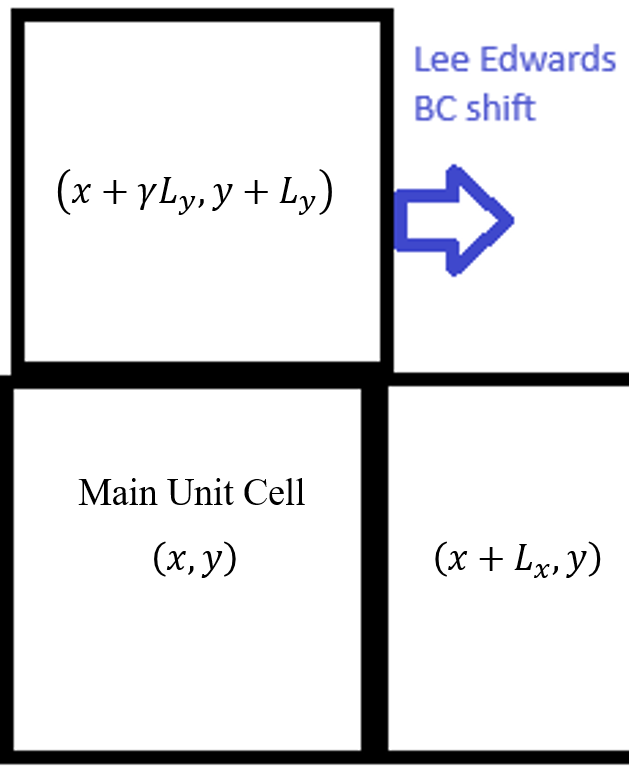
\includegraphics[scale=0.5]{leeedwards_bc.png}
	\caption{A simple illustration of the boundary conditions used for shearing. Each square represents a unit cell. The main unit cell is in the bottom left corner. Other unit cells are shifted - coordinates for each shifted are cell are labelled in the center.}
	\label{fig: leeedwards}
\end{figure}

See Fig. \ref{fig: leeedwards} for an illustration of what these looks like. 

Where $x_{ij}$ and $y_{ij}$ are the components of the vector that encodes the difference between the vector positions of $i$ and $j$. $q_{ij}$ is the tensor that captures whether the edge bounded by vertex $i$ and $j$ crosses an edge (the superscript determine which edge). 

These are the equations that we need:

\begin{align}
	\label{eqn: dEdgamma2}
	\pdv{E}{\gamma} = \sum\limits_{\alpha=1}^{F} K (A_\alpha- A_0) \pdv{A_\alpha}{\gamma} + \Gamma(P_\alpha - P_0)\pdv{P_\alpha}{\gamma}
\end{align}
We can also write the following:
\begin{align}
	\label{eqn: dedgammadr}
	\pdv[2]{E}{\gamma}{r_i^\mu} &= \sum\limits_{\alpha=1}^{F}K \pdv{A_\alpha}{\gamma} \pdv{A_\alpha}{r_i^\mu} + K (A_\alpha - A_0) \pdv{A_\alpha}{\gamma}{r_i^\mu} + \Gamma \pdv{P_\alpha}{\gamma} \pdv{P_\alpha}{r_i^\mu} + \Gamma (P_\alpha - P_0)  \pdv[2]{P_{\alpha}}{\gamma}{r_i^\mu} \\
\end{align}
Keep in mind, this gives us a vector with $2V$ elements ($V$ is the number of vertices). For the other $E$ derivative:
\begin{align}
	\label{eqn: dedgammadgamma}
	\pdv[2]{E}{\gamma} &= \sum\limits_{\alpha=1}^{F}K \pdv{A_\alpha}{\gamma} \pdv{A_\alpha}{\gamma} + K (A_\alpha - A_0) \pdv{A_\alpha}{\gamma}{\gamma} + \Gamma \pdv{P_\alpha}{\gamma} \pdv{P_\alpha}{\gamma} + \Gamma (P_\alpha - P_0)  \pdv[2]{P_{\alpha}}{\gamma}{\gamma} \\
\end{align}

Let's focus on $\pdv{P_\alpha}{\gamma}$ first. Using Eqn. \ref{eqn: perim} 
\begin{align}
	\pdv{P_\alpha}{\gamma} &= \sum\limits_{\text{CCW y-crossing edges } e \in \text{cell } \alpha}|h_{e\alpha}| \pdv{l_e}{\gamma} = \sum\limits_{\text{CCW y-crossing edges } e \in \text{cell } \alpha}|h_{e\alpha}| \pdv{\gamma} \sqrt{x_e^2 + y_e^2}\\
	\label{eqn: dpdgamma}
	&= \sum\limits_{\text{CCW y-crossing edges } e \in \text{cell } \alpha}|h_{e\alpha}| \frac{x_e^{\text{CCW}} L_y \xi(\vb{x}_e)}{\sqrt{x_e^2 + y_e^2}} = L_y\sum\limits_{\text{CCW y-crossing edges } e \in \text{cell } \alpha} \xi(\vb{x}_e) \frac{\vb{l}_e^{\text{CCW}} \cdot \hat{x} }{l_e}
\end{align}

The main challenge with this derivative is correctly determining whether the length of each edge of a cell increases or decreases in length with respect to the shear. This is not so difficult to do by hand. In fact, if we were to write out this derivative analytically, ignoring any numerical practicality concerns, we would probably write:
\begin{align}
	\label{eqn: dpdgammaanalytical}
	\pdv{P_\alpha}{\gamma} = L_y\sum\limits_{\text{CCW y-crossing edges } e \in \text{cell } \alpha} \cfrac{x_T - x_B}{l_e}
\end{align}

where $x_T$ refers to the top vertex on the crossing edge. This would be the vertex in the unit cell above the main one. $x_B$ refers to the bottom vertex on the crossing edge. This is the vertex that lives in the main unit cell. I write it differently in Eqn. \ref{eqn: dpdgamma} to account for how I do it in the actual code, where it's easier to get all the vertices in clockwise or counterclockwise order. 

However, numerically, one must either make sure each crossing edge is oriented correctly or come up with some alternative method to account for the correct sign. I use $\xi$ as a function to help do this correctly:

$\xi(\vb{l_e}) = 1$ if the edge vector starts in the primary unit cell and then goes to the unit cell above. $\xi(\vb{l_e}) = -1$ if the edge vector starts in unit cell above the primary unit cell and then comes down into the primary unit cell. I've indicated that the edge vector $\vb{l}_e$ should be oriented CCW with the superscript. This is because every cell will have two crossing edges (if it has any) and if you are traversing them in CCW order, one will point up and the other will point down. For the one pointing down, the $\xi$ adds a factor of $-1$ so that we get the sign of this derivative correct.
The summation is over ``y-crossing edges $e$ that are part of cell $\alpha$." Y-Crossing edges are the ones that cross the horizontal boundary at the top of the unit cell. I'll drop the ``h" tensor notation since it's redundant given the summation subscript given here.$l_e$ is the length of edge $e$. $x_e$ is the magnitude of the horizontal component of the vector connecting the vertices at the ends of edge $e$.  This derivative can be thought of as a force across a cutline. Recall that derivatives with respect to $L_x$ capture forces across right edge of the unit cell. However, you can take a derivative going through a vertical cutline located anywhere in the unit cell. The derivative of the perimeter of a cell with respect to $\gamma$ (in this set up)is equivalent to the derivative of the perimeter that cell with respect to vertical cutlines going through each edge that cross the y-boundary. It is debatable whether this is a useful point. Also, there is probably a decent way to incorporate Merkel/Manning's $q$ tensor for notation but it's probably not worth it. 

BIG NOTE: If we're calculating perimeters by retrieving vertices in either clockwise

Note: I'm summing over the length of the edges in the perimeter of the cell, traversing the cell counterclockwise (I compute areas by traversing the cell counterclockwise as well). This means that $x_e$ is defined as $x_e = x_i - x_j + \text{B.C.}$ where $x_i$ is the vertex you get from traversing the cell counterclockwise from $x_j$ and B.C. means ``boundary conditions." 


\begin{figure}[h!]
	\hspace{5cm}
	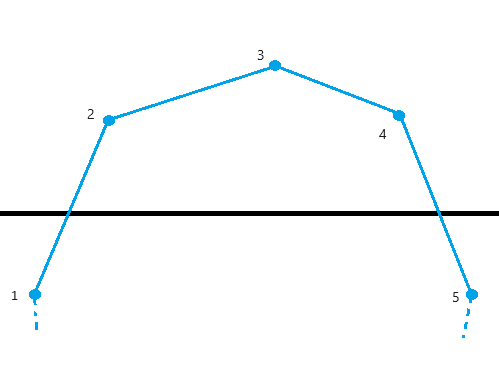
\includegraphics[scale=0.5]{sample_y_crossing_cell.png}
	\caption{A simple illustration of a cell crossing the top boundary of the packing.}
	\label{fig: crossingycell}
\end{figure}
Now we can do $\pdv{A_\alpha}{\gamma}$. Using Fig \ref{fig: crossingycell} as our case study:
\begin{align}
	\label{eqn: dadgamma}
	\pdv{A_\alpha}{\gamma} &= -\frac{1}{2}\pdv{\gamma}  \bigg\{\bigg[ x_1 \bigg(y_2 + L_y\bigg) - y_1 \bigg( x_2 + \gamma L_y\bigg)\bigg] + \bigg[ \bigg( x_2 + \gamma L_y\bigg) \bigg(y_3 + L_y\bigg) - \\ 
	&\bigg(y_2 + L_y\bigg) \bigg( x_3 + \gamma L_y\bigg)\bigg]\bigg\} + \bigg[ \bigg( x_3 + \gamma L_y\bigg) \bigg(y_4 + L_y\bigg) - \bigg(y_3 + L_y\bigg) \bigg( x_4 + \gamma L_y\bigg)\bigg]\\
	& + \bigg[ \bigg( x_4 + \gamma L_y \bigg) y_5 - \bigg(y_4 + L_y\bigg)  x_5\bigg]\bigg\}\\
	&= -\frac{L_y}{2}\bigg[ -y_1 + y_3  + L_x L_y - L_x L_y - y_2 + y_4 - y_3 + L_x L_y - L_x L_y + y_5\bigg]\\
	&= -\frac{L_y}{2}\bigg[y_{31} + y_{42} + y_{53} \bigg] \text{ Looks similar to area derivative w.r.t. vertices}\\
	&= \frac{L_y}{2}\bigg[y_{15} + y_{24}\bigg]\\
	&= \frac{L_y}{2}\bigg[(y_1 + y_2) - (y_5 + y_4)\bigg]
\end{align}

$x$ and $y$ refer to $x$ and $y$ coordinates of vertices. These are the coordinates IGNORING BOUNDARY CONDITIONS. The notation $y_{ab} = y_a - y_b$. There is a minus sign at the beginning of the left hand side for the first 3 left hand expressions because while I labelled the vertices in a clockwise manner in the image, to get a positive area, the shoelace formula needs to evaluate the vertices in a counterclockwise manner (which I did NOT do).

\begin{align}
\label{eqn: dadgammaexplicit}
\pdv{A}{\gamma} = L_y&\{[\text{avg y-coord of vertices on left y-crossing edge WOBC}]- \\& [\text{avg y-coord of vertices on right y-crossing edge WOBC}]\}
\end{align}

``WOBC" stands with ``without boundary conditions." Note: If you do account for boundary conditions, it does not affect the answer.

The more complicated ones are the second derivatives. The simplest one is the second derivative of cell areas. The first derivative of cell area with respect to $\gamma$ is dependent on only y-coordinates, which have no $\gamma$'s involved. Then:

\begin{equation}
	\label{eqn: dAdgammadgamma}
	\pdv[2]{A_\alpha}{\gamma}  = 0
\end{equation}

It's a bit more complicated for the second derivative with respect to the perimeter. From my work with calculating $\pdv{P_\alpha}{\gamma}$:

\begin{align}
	\label{eqn: dPdLx}
	\pdv{P_\alpha}{\gamma} =  L_y \sum\limits_{ \text{CCW y-crossing edges } e \in \text{cell } \alpha} \xi(\vb{l_e}) \frac{\vb{l_e}\cdot \vu{x}}{l_e} 
\end{align}

$\vb{l_e}$ refers to the vector connecting the vertices of edge $e$, defined to be pointing counterclockwise along a cell. $\xi(\vb{l_e}) = 1$ if the edge vector starts in the primary unit cell and then goes to the unit cell above. $\xi(\vb{l_e}) = -1$ if the edge vector starts in unit cell above the primary unit cell and then comes down into the primary unit cell.  You can take the second derivative with quotient rule:
\begin{align}
	\label{eqn: dPdLxdLx}
	\pdv[2]{P_\alpha}{\gamma} &= L_y^2\pdv{\gamma} \sum\limits_{ \text{CCW y-crossing edges } e \in \text{cell } \alpha} \xi(\vb{l_e})\frac{\vb{l_e}\cdot \vu{x}}{l_e} = L_y^2\sum\limits_{ \text{CCW y-crossing edges } e \in \text{cell } \alpha}  \frac{l_e - (\vb{l_e}\cdot \vu{x}) \xi(\vb{l_e})\pdv{l_e}{\gamma}}{l_e^2}\\ &= L_y^2\sum\limits_{ \text{y-crossing edges } e \in \text{cell } \alpha}  \frac{l_e}{l_e^2} - \frac{(\vb{l_e}\cdot \vu{x})^2}{l_e^3}
	= L_y^2 \sum\limits_{ \text{CCW y-crossing edges } e \in \text{cell } \alpha} \frac{\sin^2(\theta_{e})}{l_e}
\end{align}

In the last line, the $\theta_e$ refers to the angle between the crossing edge and the line that the edge is crossing (since it's crossing the ``y" boundary, the line that's getting crossed is a horizontal line, the ``+x" direction). I chose this convention to stay consistent with notation I've used for this elsewhere. 

Then, we can write the derivative we actually want as:

\begin{align}
	\label{eqn: dPdgammadgamma}
	\pdv[2]{P_\alpha}{\gamma} &= L_y^2 \sum\limits_{ \text{crossing edges } e \in \text{cell } \alpha} \frac{\sin^2(\theta_{e})}{l_e}
\end{align}

So the result is that we can simplify the expression for $\pdv[2]{E}{\gamma}$:
\begin{align}
	\label{eqn: dedgammadgamma_simplified}
	\pdv[2]{E}{\gamma} &= \sum\limits_{\alpha=1}^{F}K \bigg(\pdv{A_\alpha}{\gamma}\bigg)^2  + \Gamma \bigg(\pdv{P_\alpha}{\gamma}\bigg)^2 + \Gamma (P_\alpha - P_0)  \pdv[2]{P_{\alpha}}{\gamma} \\
\end{align}

Because of the similarity of the derivatives with respect to $\gamma$ with derivatives with respect to $L_x$ for a simple shear, this derivative will numerically implement much of the same code that the boundary term of the stress contributes. 

The trickiest derivatives will be the ones that are partial in some vertex coordinate and $\gamma$. 

\begin{align}
	\label{eqn: dedgammadr}
	\pdv{A_{\alpha}}{\gamma}{r_i^\mu} = L_y \pdv{r_i^\mu}\bigg(\bar{y}_e^{(L\alpha), WOBC} - \bar{y}_e^{(R\alpha), WOBC}\bigg)
\end{align}

In the above equation, $\bar{y}_e^{(L\alpha),WOBC}$ refers to the average of the y coordinates between the two vertices of the left edge of cell $\alpha$ that crosses the top or bottom boundaries. ``WOBC" means ``without boundary conditions." That is to say, we are not respecting boundary conditions when we take the y-coordinate of the vertices on the edges.  $\bar{y}_e^{(R\alpha ), WOBC}$ refers to the same quantity for the right edge of  the cell that  crosses the top or bottom boundary. 

\begin{equation}
	\label{eqn: ybartop}
	\bar{y}_e^{(R\alpha)} = \bigg(\frac{\vb{v}_1 + \vb{v}_2}{2}\bigg)\cdot\vu{y}
\end{equation}

In the above equation, $\vb{v}_1$ and $\vb{v}_2$ are the vertices that comprise the right edge edge that is crossing the top boundary of the box. The derivative is only non-zero if $\mu = y$ and only if vertex $i$ is part of one or both of the left and right crossing edges.


\begin{align}
	\label{eqn: dadgammadr}
	\pdv{A_{\alpha}}{\gamma}{r_i^\mu} = L_y\bigg[\frac{1}{2}\delta_{\mu,y}\bigg(\delta_{i\in L\alpha} - \delta_{i\in R\alpha}\bigg) \bigg]
\end{align}

The notation could use some work but is probably worth working out the time it takes to come up with something elegant. The $\delta_{i \in L\alpha}$ is $1$ if the vertex $i$ is in the crossing left edge and the $\delta_{i \in R\alpha}$ is $1$ if the vertex $i$ is in the crossing right edge. Otherwise, they are $0$. Note that I have written this definition from the perspective of someone who first applies the $\gamma$ derivative and then the derivative with respect to the vertex coordinate. It should be intuitive that if we apply those derivatives in the reverse order, the result will be the same. The derivative with respect to the vertex coordinate will give you the average of the pressure force acting on the two edges connected to that vertex belonging to cell $\alpha$. The $\gamma$ derivative will then take account only the edge that is crossing the boundary.
Lastly, we have the corresponding perimeter derivative. 

\begin{align}
	\label{eqn: dPdgammadr}
	\pdv{P_\alpha}{\gamma}{r_i^\mu} &=  L_y\pdv{r_i^\mu}\sum\limits_{ \text{crossing edges } e \in \text{cell } \alpha} \xi(\vb{l_e})\frac{(\vb{l_e}\cdot \vu{x})}{l_e} \\
	&= \delta_{i \in \alpha} L_y \sum\limits_{ \text{crossing edges } e \in \text{cell } \alpha} \delta_{i\in e} \xi(\vb{l_e})  \Theta(\vb{r_i})\cfrac{ l_e\delta_{x \mu} - (\vb{l_e}\cdot \vu{x}) \cfrac{(\vb{l_e}\cdot \vu*{\mu})}{l_e}}{l_e^2}\\
	&= \delta_{i \in \alpha} L_y \sum\limits_{ \text{crossing edges } e \in \text{cell } \alpha} \delta_{i\in e} \xi(\vb{l_e}) \Theta(\vb{r_i})\cfrac{ l_e^2\delta_{x \mu}  - (\vb{l_e}\cdot \vu{x}) (\vb{l_e}\cdot \vu*{\mu})}{l_e^3}\\
\end{align}

As before $\xi(\vb{l_e})$ is $1$ if $\vb{l_e}$ points up (in the positive $\vu{y}$ direction) and $-1$ otherwise. $\Theta(\vb{r_i})$ is $1$ if vertex $i$ is the CCW vertex on edge $e$ and $-1$ otherwise. For the second term, the derivative with respect to the vertex pulls out the magnitude of the $\mu$ component of the y-crossing edge. 
So let's summarize. First, we can discuss:

\begin{equation}
	\label{eqn: dedgammadgamma_resum}
	\pdv[2]{E}{\gamma} = \sum\limits_{\alpha=1}^{F}K \pdv{A_\alpha}{\gamma} \pdv{A_\alpha}{\gamma} + \Gamma \pdv{P_\alpha}{\gamma} \pdv{P_\alpha}{\gamma} + \Gamma (P_\alpha - P_0)  \pdv[2]{P_{\alpha}}{\gamma}{\gamma}.
\end{equation}

$\pdv{A_\alpha}{\gamma}$ can be defined as:
\begin{align}
	\label{eqn: dadgamma_resum}
	\pdv{A_\alpha}{\gamma} =  L_y\bigg(\bar{y}_e^{(L\alpha)} - \bar{y}_e^{(R\alpha)}\bigg)
\end{align}
where the overbar refers to an average of the y-coordinates of the vertices on edge $e$. Because derivatives on $\gamma$ in this simple shear case act only on the $x$ coordinate, $\pdv[2]{A_\alpha}{\gamma} = 0$. 


\begin{align}
	\label{eqn: dAdgamma_resum}
	\pdv[2]{A_\alpha}{\gamma} &= 0.
\end{align}

For the perimeter:
\begin{align}
	\label{eqn: dPdgamma_resum}
	\pdv{P_\alpha}{\gamma} &= L_y \sum\limits_{ \text{crossing edges } e \in \text{cell } \alpha} \xi(\vb{l_e}) \cos(\theta_{e}).
\end{align}


\begin{align}
	\label{eqn: dPdgammadgamma_resum}
	\pdv[2]{P_\alpha}{\gamma} &= L_y^2 \sum\limits_{ \text{crossing edges } e \in \text{cell } \alpha} \frac{\sin^2(\theta_{e})}{l_e}
\end{align}

$\theta_e$ is the angle between the crossing edge and the x-axis. We need more derivatives to discuss

\begin{align}
	\label{eqn: dedgammadr_resum}
	\pdv[2]{E}{\gamma}{r_i^\mu} &= \sum\limits_{\alpha=1}^{F}K \pdv{A_\alpha}{\gamma} \pdv{A_\alpha}{r_i^\mu} + K (A_\alpha - A_0) \pdv{A_\alpha}{\gamma}{r_i^\mu} + \Gamma \pdv{P_\alpha}{\gamma} \pdv{P_\alpha}{r_i^\mu} + \Gamma (P_\alpha - P_0)  \pdv[2]{P_{\alpha}}{\gamma}{r_i^\mu}. \\
\end{align}

The derivatives that are partial in $\gamma$ and a vertex coordinate are:

\begin{align}
	\label{eqn: dadgammadr_resum}
	\pdv{A_{\alpha}}{\gamma}{r_i^\mu} = L_y\bigg[\frac{1}{2}\delta_{\mu,y}\bigg(\delta_{i\in R\alpha} - \delta_{i\in L\alpha}\bigg) \bigg]
\end{align}

and 
\begin{align}
	\label{eqn: dPdgammadr_resum}
	\pdv{P_\alpha}{\gamma}{r_i^\mu} &=  \delta_{i \in \alpha} L_y \sum\limits_{ \text{crossing edges } e \in \text{cell } \alpha} \delta_{i\in e} \xi(\vb{l_e}) \Theta(\vb{r}_i)\cfrac{ l_e^2\delta_{x \mu} - (\vb{l_e}\cdot \vu{x}) (\vb{l_e}\cdot \vu*{\mu})}{l_e^3}\\
\end{align}

\section{Dealing With $K$'s Pressure Units}

$K$ has funny units in the AGPerim version of the tissue class because the pressure is defined as:

\begin{equation}
	\Pi_{\alpha} = K' \bigg(\frac{A_{\alpha}}{A_0} - 1\bigg)
\end{equation}

This means $K'$ has units of pressure which is not how my equations above were formulated. We can related $K$ to $K'$ with 
\begin{equation}
K' = K A_0
\end{equation}

\begin{align}
	\label{eqn: dedgammadr22}
	\pdv[2]{E}{\gamma}{r_i^\mu} &= \sum\limits_{\alpha=1}^{F} \frac{K'}{A_0} \pdv{A_\alpha}{\gamma} \pdv{A_\alpha}{r_i^\mu} + \frac{K'}{A_0} (A_\alpha - A_0) \pdv{A_\alpha}{\gamma}{r_i^\mu} + \Gamma \pdv{P_\alpha}{\gamma} \pdv{P_\alpha}{r_i^\mu} + \Gamma (P_\alpha - P_0)  \pdv[2]{P_{\alpha}}{\gamma}{r_i^\mu} 
\end{align}
\begin{align}
	\label{eqn: dedgammadgamma_simplified22}
	\pdv[2]{E}{\gamma} &= \sum\limits_{\alpha=1}^{F}\frac{K'}{A_0} \bigg(\pdv{A_\alpha}{\gamma}\bigg)^2  + \Gamma \bigg(\pdv{P_\alpha}{\gamma}\bigg)^2 + \Gamma (P_\alpha - P_0)  \pdv[2]{P_{\alpha}}{\gamma} \\
\end{align}

\begin{align}
	\label{eqn: Hessian2}
	\pdv[2]{E}{r_j^\nu}{r_i^\mu} &= \sum\limits_{\alpha=1}^{F}\frac{K'}{A_0} \pdv{A_\alpha}{r_j^\nu} \pdv{A_\alpha}{r_i^\mu} + \frac{K'}{A_0} (A_\alpha - A_0) \pdv[2]{A_\alpha}{r_j^\nu}{r_i^\mu} + \Gamma \pdv{P_\alpha}{r_j^\nu} \pdv{P_\alpha}{r_i^\mu} + \Gamma (P_\alpha - P_0)  \pdv[2]{P_{\alpha}}{r_j^\nu}{r_i^\mu} \\
	= H_{ij}^{\mu \nu}
\end{align}
\end{document}


